% Chapter 6

\chapter{Schematic \& PCB Layout} % Main chapter title

\label{Chapter6} % For referencing the chapter elsewhere, use \ref{Chapter1} 

\begin{figure}[!htb]
	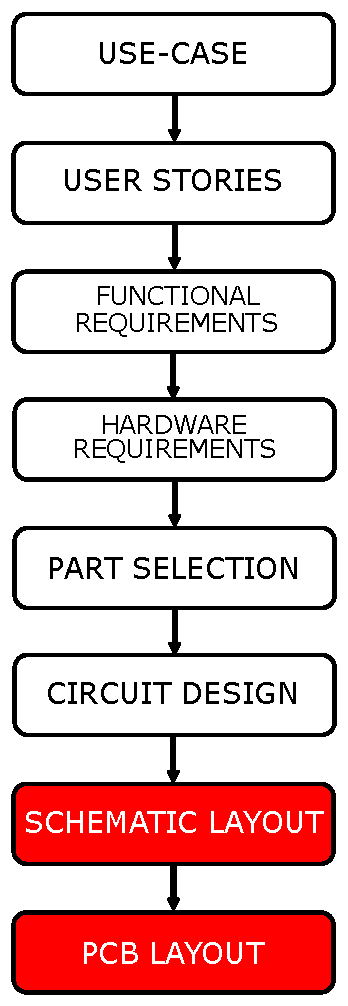
\includegraphics[width=0.5\linewidth]{Figures/layout_table.pdf}\centering
	\label{fig:layout}
\end{figure}

%----------------------------------------------------------------------------------------
	This section provides a detailed overview of the process and findings of the circuit designs to create the schematic designs, as well as the derivation of the PCB from the schematic designs. This includes: (\ref{chap6sec1} the schematic design errors and (\ref{chap6sec2}) testing, (\ref{chap6sec3}) PCB concept drawings, (\ref{chap6sec4}) the PCB footprint design, (\ref{chap6sec5}) the layout of the PCB, (\ref{chap6sec6}) the routing of the PCB and (\ref{chap6sec7}) any major challenges which were faced.\\

%----------------------------------------------------------------------------------------
%	SECTION 1
%----------------------------------------------------------------------------------------

\section{Errors in the Schematic Designs}
\label{chap6sec1}

There were originally as many as 900 errors found in the design project after compiling. A large number were removed by disabling the warning given for off-grid objects. This left about 500 errors which needed to be solved individually. The following list describes the major errors and how they were solved.

\begin{itemize}
\item no driving source; this was corrected in a number of different ways. In some situations it required signal connections at each end to be related (input to output) and not the same. In other cases it required adding in either a power rail or a ground to the affected component to fix the driving source. 
\item only one pin connection; this was solved by going to the causing net label, recreating it and placing it in the desired location. 
\item a certain component had a mix of I/O pins and output pins (or power pins); this was solved by changing the pin types of the affecting pins to match the required in type. This was an easy solve in most cases however some were more tricky and required work overall several schematics. 
\end{itemize}

A few other small changes were made to the schematics to improve the aesthetic and readability of the documents, as well as saving the amount of components needed. All of the resistor pull-ups for the I2C connections were moved to the Signal Connections schematic, which saved a large number of resistors and space. Also, the solder jumpers were removed and replaced with ones which were professionally created, so that they would give no errors.

%----------------------------------------------------------------------------------------
%	SECTION 2
%----------------------------------------------------------------------------------------

\section{Testing the Schematic Components}
\label{chap6sec2}

The initial testing was started before the schematic were completed and before the design of the PCB. The first components which were tested were the voltage regulators and the flip-flops being used within the Power Control circuitry. It was vital that the correct voltage was being read out of the flip-flop to ensure that the correct pins were being wired. It was also vital that the correct lines were being shutdown if necessary so that the security of the circuitry could be verified. The circuitry was put together and tested on a small breadboard with both a resistor and a capacitor in certain positions to obtain the required voltage. Once the expected reading was achieved the circuit was copied into the schematic for the Power Control circuitry and was replicated a number of times for all the required power rails. Figure \ref{fig:power_circuit} shows the power circuit used with the smaller IC being the voltage regulator and the larger IC being the flip-flop.

\begin{figure}
	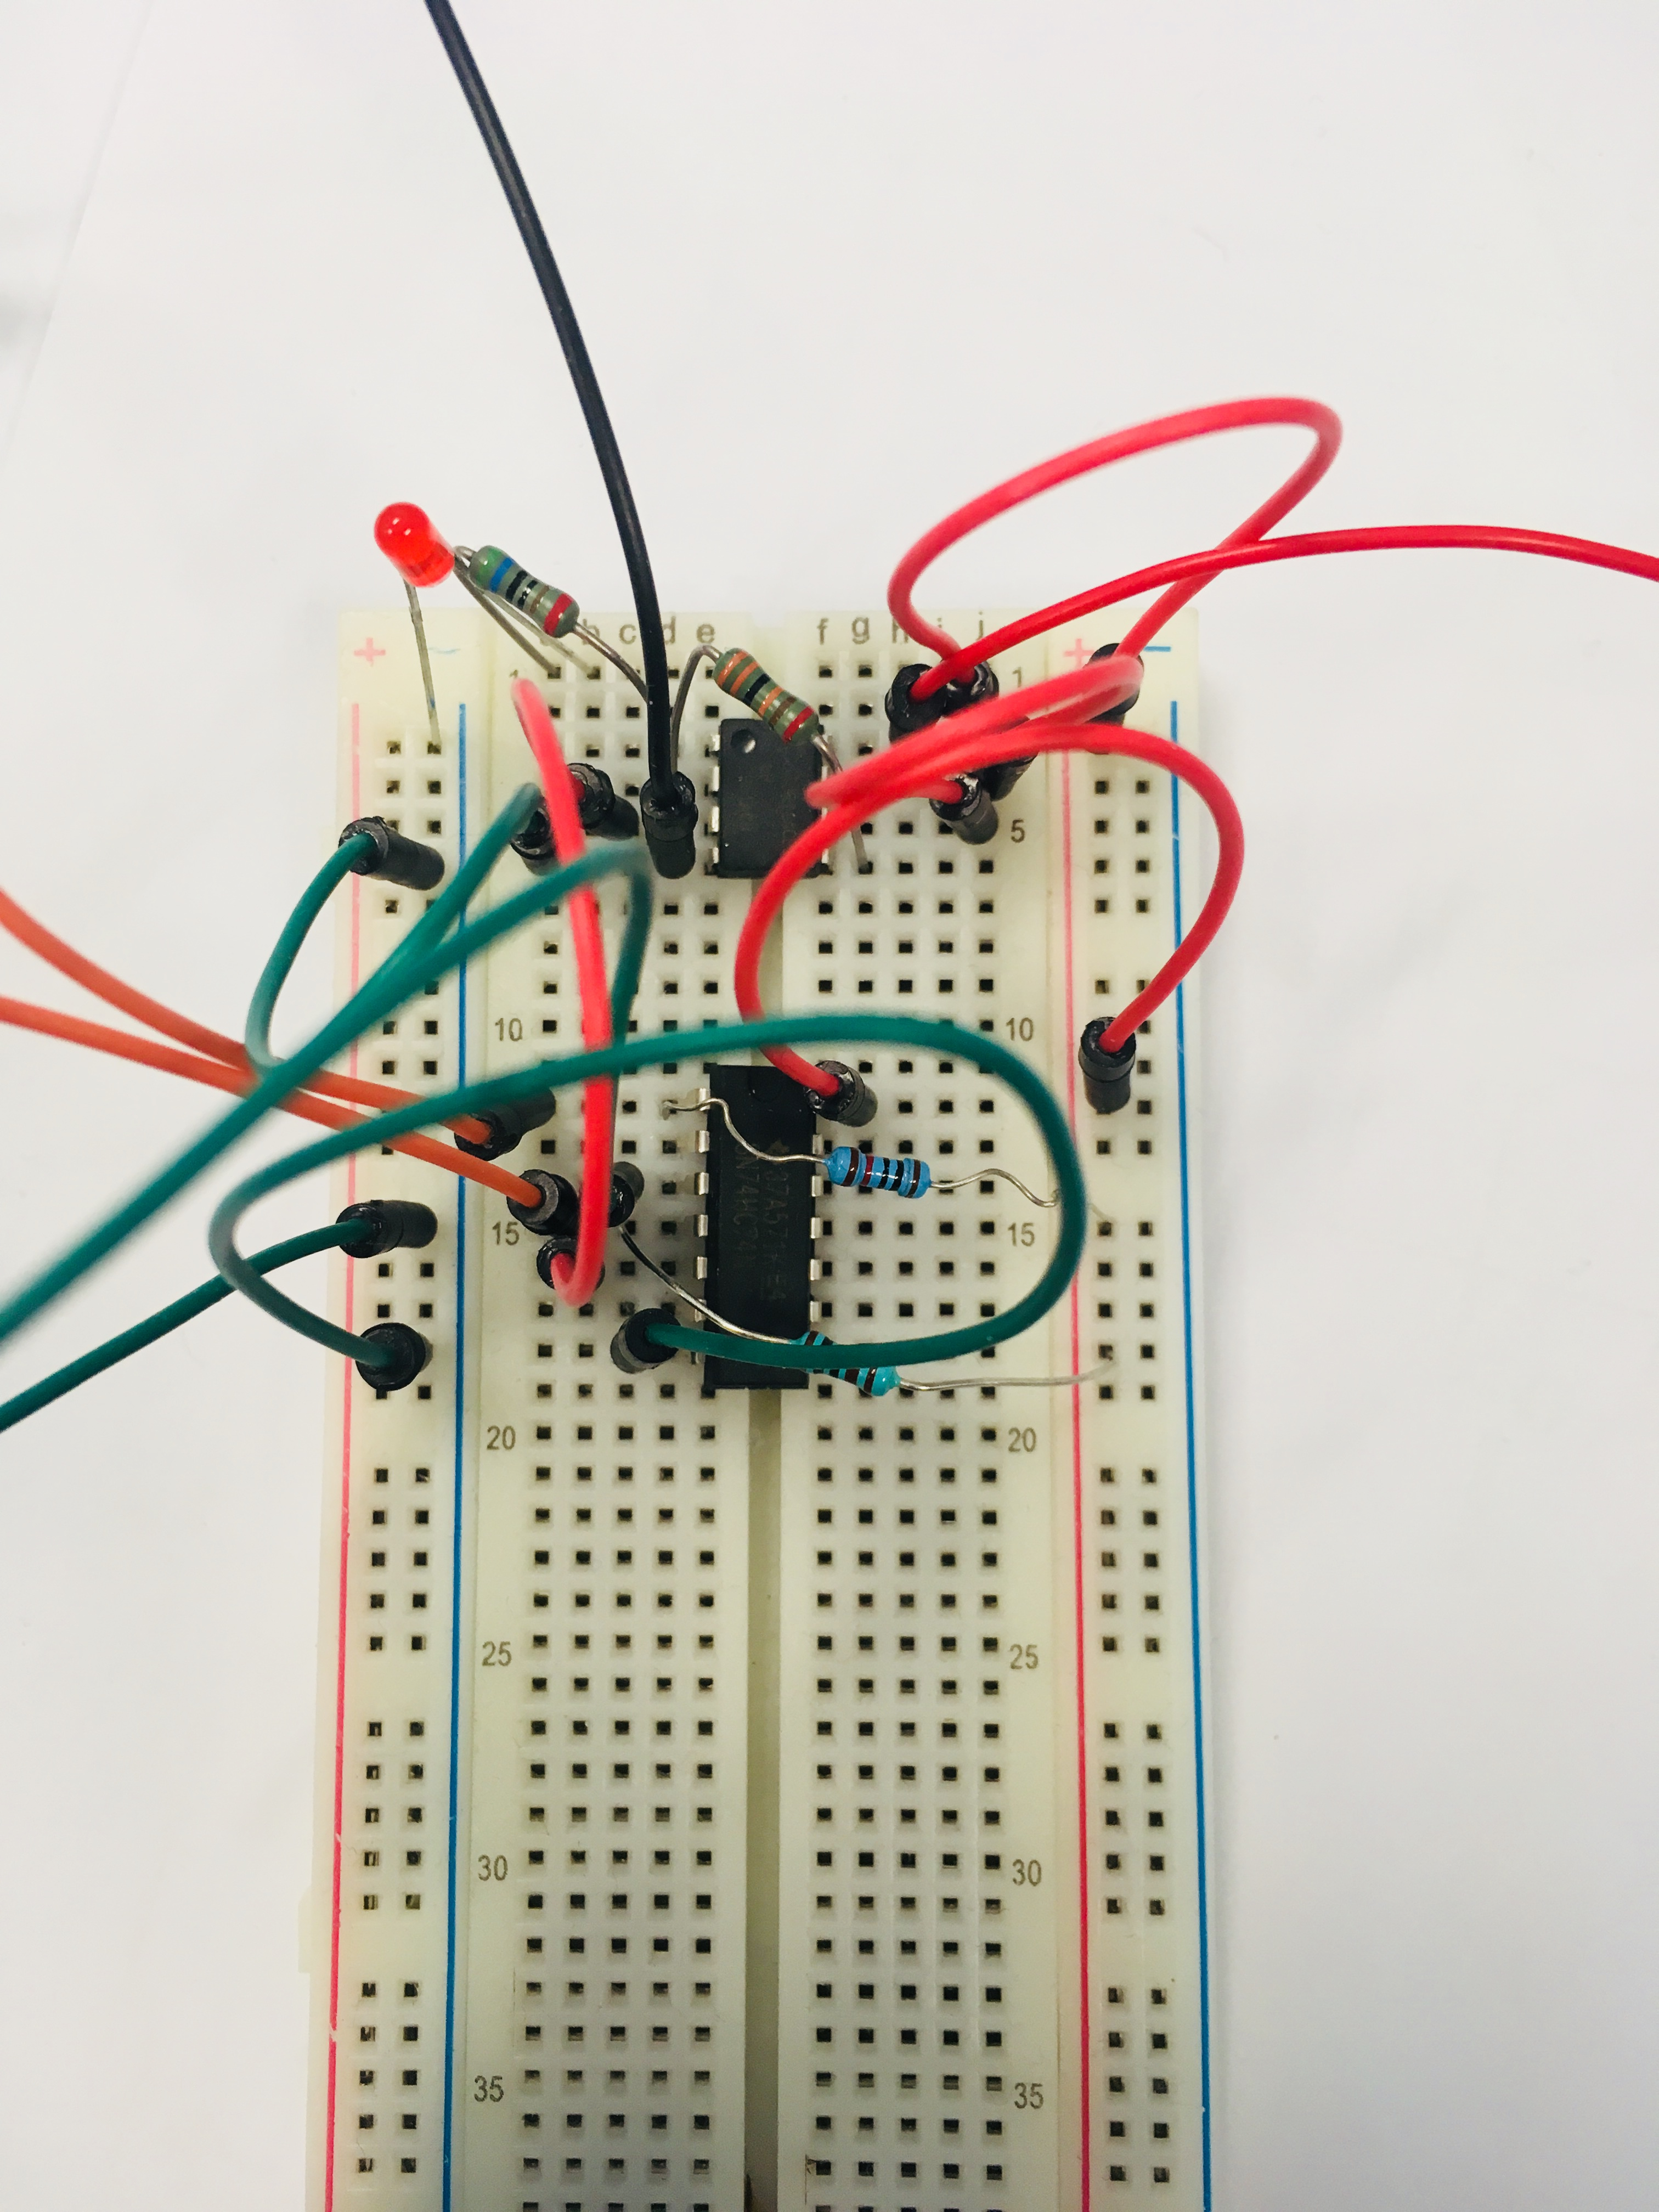
\includegraphics[width=0.5\linewidth]{Figures/powercircuit.jpg}\centering
	\caption{Image of test power circuit}
	\label{fig:power_circuit}
\end{figure}


%----------------------------------------------------------------------------------------
%	SECTION 3
%----------------------------------------------------------------------------------------

\section{PCB Concept}
\label{chap6sec3}

The PCB layout originated from early concept designs created by Paul Gardner-Stephen. This multi-layered design was used to visualise the placement of every major component within the phone. Figure \ref{fig:Concept} displays the concept design on the top layer. 

\begin{figure}
	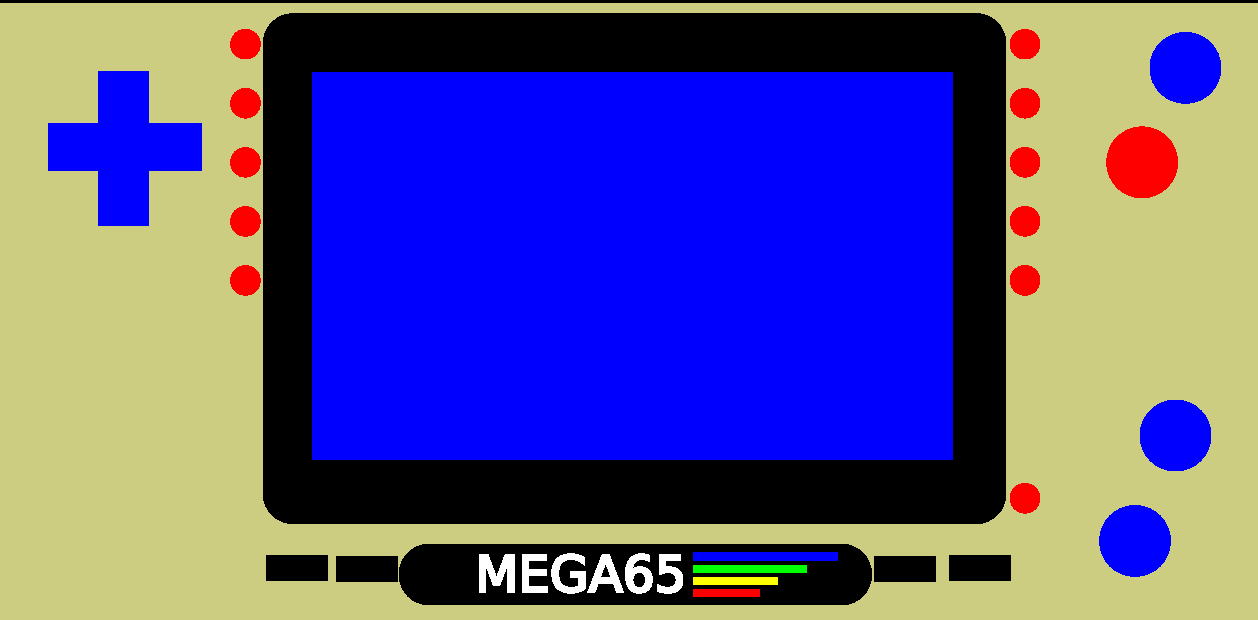
\includegraphics[width=\linewidth]{Figures/handset-layout-v1.pdf}
	\caption{Initial PCB Concept}
	\label{fig:Concept}
\end{figure}

	The following figures display the lower layers of the concept, detailing the location of most of the vital components. 

\begin{figure}
	\includegraphics[width=\linewidth]{Figures/handset-layout-v1-no-cover.pdf}
	\caption{Concept PCB with no cover}
	\label{fig:nocover}
\end{figure}

\begin{figure}
	\includegraphics[width=\linewidth]{Figures/handset-layout-v1-no-PCB-no-cover.pdf}
	\caption{Concept detailing PCB component placement }
	\label{fig:nopcb}
\end{figure}

%----------------------------------------------------------------------------------------
%	SECTION 4
%----------------------------------------------------------------------------------------

\section{PCB Footprint Design}
\label{chap6sec4}

	Most of the components were either downloaded from the manufacturer's approved source (eg. Digikey) or SnapEDA, components which didn't have footprints or where the footprints had incorrect dimensions were created manually using the footprint editor in Alitum. The footprints were created by following the recommended PCB outline in the desired component's datasheet. There were a few components where the datasheet was unavailable and hence the footprints were created using precise measurements of the actual item. The following list describes the footprints which were created without a datasheet, and how they were created;

\begin{itemize}
\item The footprints for the silicon moulds for the push buttons were designed in Altium using a pre-existing official footprint used for the design of the Nintendo Gameboy. This larger footprint was modified into the separate components of the DPAD buttons, the blue push buttons and the rectangular black push buttons.
\item The footprint for the modem connector was created by measuring the dimensions of the physical component. This connection part was then added to the recommended PCB layout of the modem, which was created from the datasheet. 
\end{itemize}

%----------------------------------------------------------------------------------------
%	SECTION 5
%----------------------------------------------------------------------------------------

\section{PCB Layout}
\label{chap6sec5}

	The start of the PCB Design process begun with a graphical editor being used to create a mockup of the MEGA65 phone. This mockup included precise measurements of the height and width of the device as well as the location of all of the major components required for the device, including the FPGA pins and the 4G Modems. The mockup was used as the template for the PCB board with all of the measurements copied into the program. \\
	Once the schematic designs had been completed the PCB board was adjusted in Alitum to accomodate four layers. This was completed by going into Layer Stack Manager in Alitum and adding in two more signal layers. All of the schematic designs were then added into the PCB file and on top of the mockup. \\
The next stage of the process involved using the mockup (Figure \ref{fig:nopcb}) to place the required components in their suitable positions. This process took a while to complete as some components were required to be realigned or moved to a completly different position. Some component footprints also had small positioning holes, which interfered with components in the same position on the opposite side of the board. This also required realignment of a number of components. Figure \ref{fig:Initial_PCB} displays one of the initial PCB layouts of the board, before the routing stage. Note that this early design doesn't include a lot of the components, nor most of them are not in thieir correct positions.\\

\begin{figure}
	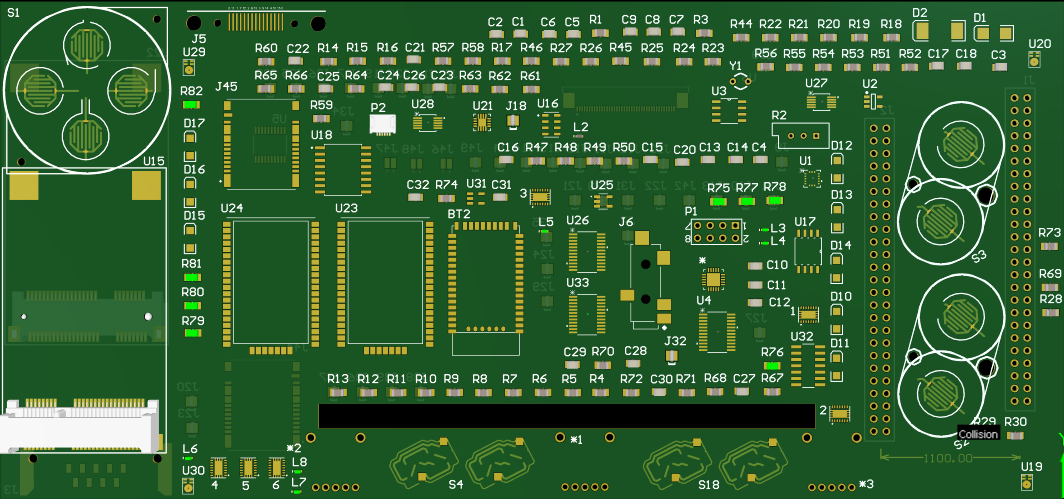
\includegraphics[width=\linewidth]{Figures/PCB.png}
	\caption{Initial PCB Layout}
	\label{fig:Initial_PCB}
\end{figure}

	It was decided near the beginning of the process that most of the ICs which would be located within the inner part of the board, would have to be positioned on the bottom layer of the board. This was needed to allow the LCD screen to lie flush with the board. It was also decided that the solder jumpers could be placed on the top side of the board below the LCD screen, as they would take up minimal height.\\

\subsection{Component Placement}
	Once all the components were placed in their relative positions they were precisely aligned into their correct positions based upon the prototype on the bench, and the concept which was made digitally. The FPGA pins were aligned first along with the connectors for both the LCD screen and the touch screen. It was essential that the large rectangular whole at the bottom of the phone was also the right width and height from the bottom of the device so that the LCD and touch ribbons would meet the connector points on the board. Figure \ref{fig:component_placement} shows the dimensions for the touch screen connector. 

\begin{figure}
	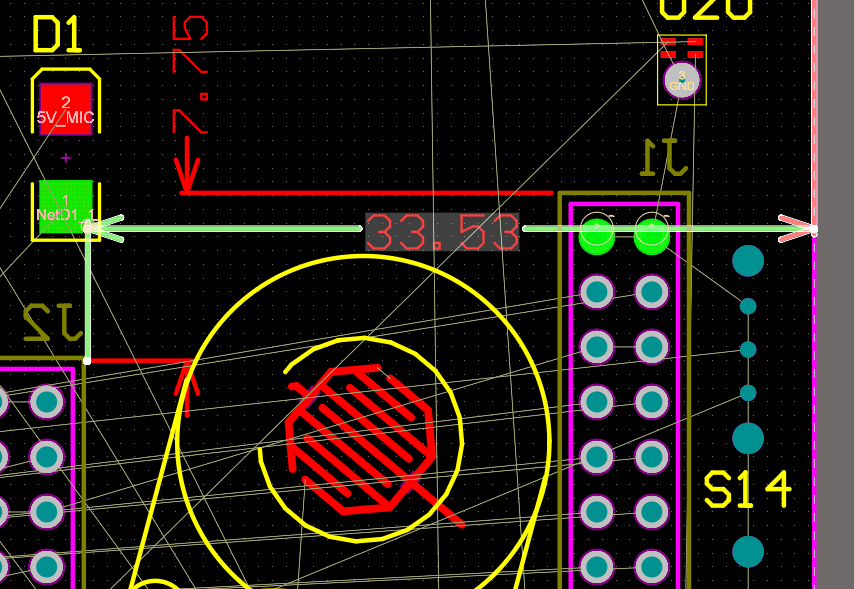
\includegraphics[width=\linewidth]{Figures/component_placement.png}\centering
	\caption{LCD Screen Dimensioning}
	\label{fig:component_placement}
\end{figure}

%----------------------------------------------------------------------------------------
%	SECTION 6
%----------------------------------------------------------------------------------------

\section{PCB Routing}
\label{chap6sec6}

	Before the routing stage of the board development could begin there were a number of errors which needed to be addressed. To begin, some of the footprints weren't working correctly when imported over to the PCB file. Some of these issues were solved by going back into the schematic files and making sure that all the correct footprints were in place, for every component. Another error was that 

%----------------------------------------------------------------------------------------
%	SECTION 7
%----------------------------------------------------------------------------------------

\section{Challenges}
\label{chap6sec7}

	There were a number of challenges with designing the PCB board, mainly to do with the vast majority of components needed to be routed. Another challenge was discovered in the fact that the aim was to have a six-layered board, which in itselt is highly sophiscated. It was decided early on that the majority of the tricky PCB routing and design would be completed by a professional PCB designer in Germany.\\
Another challenge was found in working out the dimensions of the PCB as well as the component placement. Due to the size requirements of the board there was not a lot of room to spare with many components sitting flush with one another and required precise measurements to fit. \\
The PCB footprint design also provided a number of challenges with some of the components either not having datasheets, or their datasheets not showing the recommended PCB layout. In these cases a physical copy of the components was obtained and precisely measured before designing the component's footprint.






%----------------------------------------------------------------------------------------





